\chapter{Preliminary Work}
	
	% Various work done to build experience with interconnect simulation, SpiNNaker,
	% built some useful tools (wiring) and to test the principle of adding
	% connections (small world).
	
	The preliminary work conducted so far aims to explore some of the practical
	issues faced when designing interconnection networks. The work focuses on the
	SpiNNaker architecture whose advanced state of development makes it an
	appropriate target for realistic experimentation.
	
	The first section describes an experiment conducted to determine the way in
	which the choice of technologies on which an interconnection network is built
	can affect its performance. As well as performance considerations, this choice
	also has implications for the practicalities of constructing real systems. The
	second section describes work which studies the practical issues faced when
	wiring up SpiNNaker's chosen interconnect. The chapter concludes with an
	experiment to test a simple extension to the SpiNNaker interconnect topology.
	The proposed topology uses semi-random links to improve its performance while
	still accounting for the practical issues involved in assembly.
	
	% Rly?
	%\section{PCI-Express and High-Speed Serial}
	%	
	%	One way of getting data from one part of the machine to the other would be
	%	not to just dump it through another link but to pull it straight out into a
	%	conventional computer via PCI-Express and then maybe re-route it with
	%	fancier software or via the web.
	%	
	%	\subsection{PCI-Express}
	%		
	%		What is PCI-Express? How does it work? Where is it found?
	%	
	%	\subsection{High Speed Serial on FPGA}
	%		
	%		What is an FPGA? We have one on the boards. FPGAs contain hard-wired
	%		blocks which do special purpose things, one such job is to do PCI-Express.
	
	\section{SpiNNaker Interconnect Modelling}
		
		\label{sec:interconnect-modelling}
		
		% In order to understand the effects of inserting non-uniformity to the
		% SpiNNaker Interconnect caused by the high speed links.
		
		An important factor in designing interconnection networks is the technology
		used to implement the links in the network. These choices influence the
		network's performance as they determine the costs involved in sending a
		message across a link. This in turn can, for example, affect the way packets
		need to be routed to make optimal use of the system's resources.
		
		At the chip-to-chip level, the SpiNNaker system is homogeneous with
		identical links connecting chips to their (also identical) neighbours.
		Unfortunately, this homogeneity is broken when signals need to cross between
		boards. The board-to-board links concentrate multiple chip-to-chip signals
		onto a small number of high-speed serial links to reduce the cost of wiring.
		
		Though the board-to-board connections are logically transparent, they
		inevitably result in some additional latency at the board boundaries. Figure
		\ref{fig:boardToBoardSchematic} shows a high-level schematic of the
		board-to-board links. At both ends of the link, additional processing and
		buffering is required. Each link must collect packets from the attached
		chips into frames which are then sent across the high-speed serial link,
		requiring buffering at each stage. All of these steps incur additional
		latency over a direct connection between two chips.
		
		\begin{figure}
			\center
			\begin{tikzpicture}[thick,minimum height=2em,node distance=1em]

	\node (chip a)
		[draw,minimum size=1.8cm]
		{Chip};
	\node (fpga a)
		[matrix, draw, right=2em of chip a, inner sep = 1ex]
		{
				\node (in buf)
					[draw]
					{Buffer};
				\node (packet asm)
					[draw, right=of in buf]
					{Frame Assembly};
				\node (transceiver a)
					[draw, right=of packet asm]
					{Transmit Buffer};
				\draw [->] (in buf) to (packet asm);
				\draw [->] (packet asm) to (transceiver a);
				\\
		};
	
	\node [above=0 of fpga a] {FPGA};
	
	\draw [->] (chip a) to (in buf);
	
	\node (chip b)
		[draw,minimum size=1.8cm,below=2.5em of chip a]
		{Chip};
	
	\node (fpga b)
		[matrix, draw, right=2em of chip b, inner sep = 1ex]
		{
				\node (in buf)
					[draw]
					{Buffer};
				\node (packet asm)
					[draw, right=of in buf]
					{Frame Disassembly};
				\node (transceiver b)
					[draw, right=of packet asm]
					{Receive Buffer};
				\draw [<-] (in buf) to (packet asm);
				\draw [<-] (packet asm) to (transceiver b);
				\\
		};
	
	\node [above=0 of fpga b] {FPGA};
	
	\draw [<-] (chip b) to (in buf);
	
	\draw [->] (transceiver a.east) -- +(1cm,0)
	      |- (transceiver b.east);
	
	\node (label a)
		[left=of chip a]
		{Board A};
	
	\node (label b)
		[left=of chip b]
		{Board B};
	
	\draw [help lines]
	      ([xshift=-0.5em]$(label a.west)!0.5!(label b.west)$)
	   -- ([xshift=2.5em]$(fpga a.east)!0.5!(fpga b.east)$)
	      ;

\end{tikzpicture}

			\caption[SpiNNaker high-speed serial board-to-board
			link schematic.]{Simplified schematic of the processing stages encountered by a
			packet crossing between boards connected via a high-speed serial link.}
			\label{fig:boardToBoardSchematic}
		\end{figure}
		
		The real-time nature of SpiNNaker's simulations means that the latency of
		packets in the system can be critical to the simulation's correctness. If a
		packet takes too long to be delivered this counts as a failure of the
		system. Indeed, packets travelling across the entire system may have to pass
		through a number of these links potentially incurring a high latency
		penalty.
		
		Because latency between pairs of chips is no longer uniform, this violates
		the assumptions made by the routing schemes currently in use. The cost of
		this mistaken assumption is not known and one of the aims of this work was
		to measure its impact.
		
		\subsection{Simulation}
			
			To study the effects of the board-to-board links, a simplified simulation
			of SpiNNaker's interconnect was built. The simulated model was based on
			the work presented by Navaridas et al. in \cite{navaridas09} but using an
			alternative simulator written in Python to speed up development. As the
			high-speed serial links are under active development, they have been
			modelled using the expected latency values for the completed system.
			
		\subsection{Results}
			% Found a significant increase in average latency. Maybe this could be
			% overcome by making more use of that added processing time by jumping on
			% further ahead? Further simulation needs to be done anyhow...
			
			Simulations of systems containing a toroid of $4\times4$ threeboards (48
			boards, 2,304 chips) were performed under various conditions.
			
			\subsubsection{Packet Latency}
			
				To test the effect of board-to-board links on packet latency, the
				network was simulated with each chip generating a packet every CPU
				cycle, with a probability of 1\%, to uniform-random destinations. The
				latency added by the serial links can be seen in figure
				\ref{fig:min-time-for-hops} where the minimum packet latency is shown
				against the number of links (hops) used by a packet. The system is also
				shown as if using only chip-to-chip links, with realistic high-speed
				serial links and with high-speed serial links with exaggerated latencies
				(for illustrative purposes) as board-to-board links.
				
				\begin{figure}
					\centering
					
					\begin{subfigure}[t]{0.45\textwidth}
						\centering
						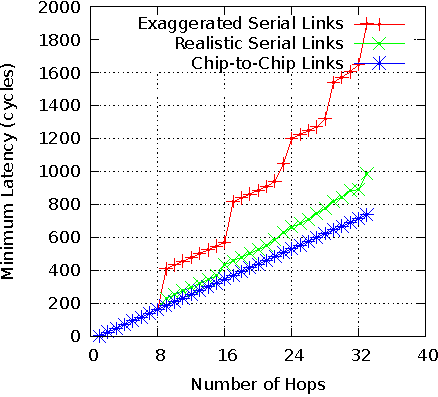
\includegraphics[width=\textwidth]{figures/min-time-for-hops}
						\caption{Minimum latencies.}
						\label{fig:min-time-for-hops}
					\end{subfigure}
					\begin{subfigure}[t]{0.45\textwidth}
						\centering
						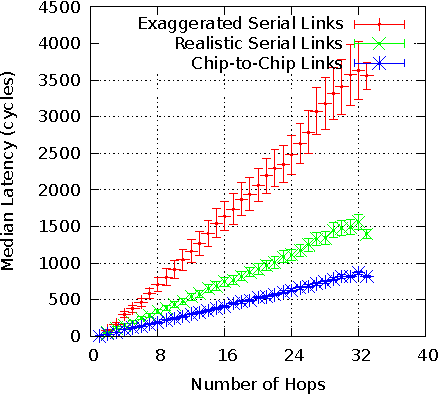
\includegraphics[width=\textwidth]{figures/median-time-for-hops-with-errbars}
						\caption{Median latencies, error bars $=
						0.1\times\textrm{Inter-Quartile Range}$.}
						\label{fig:median-time-for-hops-with-errbars}
					\end{subfigure}
					
					
					\caption{Packet latencies for various types of board-to-board
					links.}
					\label{fig:time-for-hops}
				\end{figure}
				
				Steps can be seen every time the number of hops passes a multiple of 8,
				the number of consecutive chips in any single dimension on a board,
				after which a board-to-board link is crossed causing increased latency.
				This step change can be seen clearly in the exaggerated links but is
				also visible in realistic links.
				
				An extra step appears at 28 hops, the cause of which is not currently
				known by the author.
				
				% 2-of-7 gradient: 27.2751
				% S-ATA gradient: 49.209
				% Extreme gradient: 118.013
				
				The median latency of an $n$-hop path increases smoothly as shown in
				figure \ref{fig:median-time-for-hops-with-errbars} as the probability of
				crossing a boundary increases with the number of hops carried out. From
				the gradient of these lines it can be seen that the realistic serial links
				result in an 80.4\% latency overhead.
			
			\subsubsection{Na\"ive Routing Effects}
				
				The routing scheme used by current SpiNNaker simulations is based on
				dimension order routing. This scheme assumes that all `hops' take the
				same amount of time in order to generate routes with minimal-latency.
				This assumption breaks down in heterogeneous systems.
				
				Figure \ref{fig:packet-latency-unloaded} shows how the latencies vary
				across an idle system from a single point. It can be seen that where board
				boundaries (shown in white) are crossed there is a general increase in
				latency. Because of this, the contours are visibly distorted from the
				expected hexagonal shape. This is particularly visible at the bottom left
				and top right of the figure.
				
				\begin{figure}
					\centering
					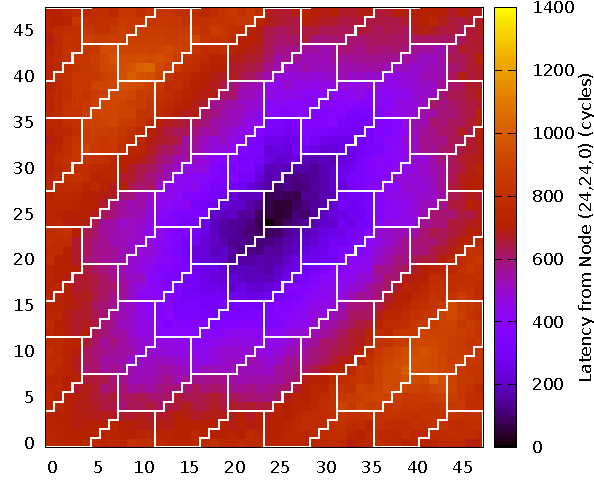
\includegraphics[width=0.7\textwidth]{figures/packet-latency-unloaded.pdf}
					
					\caption[Heat-map of average packet latency.]{Heat-map of average
					packet latency to each chip from the central chip. Note: a skewed
					perspective is used.}
					
					\label{fig:packet-latency-unloaded}
				\end{figure}
				
				A step in latency is also visible within individual boards as can be
				seen in figure \ref{fig:packet-latency-closeup-exaggerated}. Here there
				are clear edges where dimension order routing traverses the dimensions
				in an order which incurs an extra board crossing. This effect is visible
				as a step-change in latency along the diagonals of the upper-right
				boards.
		
				\begin{figure}
					\center
					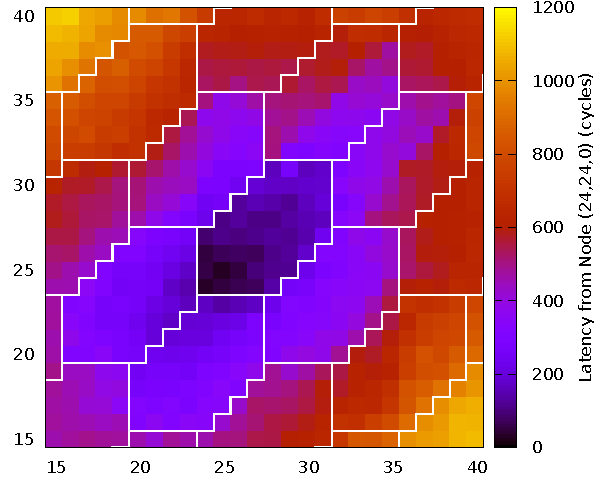
\includegraphics[width=0.7\textwidth]{figures/packet-latency-closeup-exaggerated.pdf}
					
					\caption[Latency to a subset of chips with exaggerated board-to-board
					latency.]{Latency to each chip from the central chip (24,24) to a
					section of a $48\times{}48$ system. The serial latency in this system
					has been exaggerated to aid visibility but the effect is still present
					with realistic latencies.}
					
					\label{fig:packet-latency-closeup-exaggerated}
				\end{figure}
		
		\subsection{Conclusions}
			
			Though at first sight the 80.4\% latency penalty seems severe, for
			SpiNNaker's target of SNNs running at 1 ms time steps this is not fatal.
			The new median latency is still only around 7.5 $\mu$s for the longest
			possible path, very much smaller than 1 ms deadline.  For much the same
			reason, the effects of na\"ively routing packets should also not affect
			current simulation schemes significantly.
			
			% XXX: Do gossiping algorithms care about latency?
			
			For other more latency sensitve applications such as finer-grained neural
			simulations, the increase in latency due to poor routing choices may still
			be problematic.
			
			It is worth noting that the simulations carried out were limited in size,
			duration and traffic complexity by the performance of the simulator. An
			improved simulator would allow larger models to be simulated using more
			realistic networks. One possible approach is to extend the simulator used
			by Navaridas et al. and this is discussed in \S\ref{sec:simulator-improvement-plan}.
		
	
	\section{Wiring-Up Large SpiNNaker Machines}
		
		\label{sec:wiring-up-large-spinnaker-machines}
		
		% A practical constraint on any interconnect is that it should be possible to
		% wire it up. In particular constraints exist on both on wire length and the
		% practical difficulty of connecting up the wires into the correct places.
		% Computers usually placed in racks. Tool can be used to study wiring
		% constraints of new links.
		
		One of the practical constraints on the topologies is the use of wires to
		connect parts of the system together.  Chief amongst these concerns are the
		following:
		
		\begin{description}
			
			% TODO: Explain this one since I moved the spinnaker machine description
			% elsewhere
			\item[Wire Cost] The choice of cabling used has a direct impact on the
			financial cost of the wiring. Higher quality materials or increased
			numbers of wires can substantially drive up the cost of the cable and
			connectors required.
			
			\item[Wire Length] Long wires have higher capacitances than short ones
			limiting the rate at which data can be transmitted.
			
			\item[Wiring Complexity] Ultimately the system will need to be assembled
			(usually) by hand so keeping wiring patterns simple is important to
			prevent wiring mistakes.
			
		\end{description}
		
		The SpiNNaker interconnect topology was studied to confirm the existence of
		a practical wiring scheme which satisfies all of the above properties. The
		principles of the machine's construction suggested by Davidson
		\cite{davidsonWiring} and Furber \cite{furber13email} were used as the basis
		for a tool used to model and experiment with possible configurations. This
		section explains the mapping developed and how it meets the above
		requirements. Finally, the section concludes with a description of the tool
		and the future work which remains.
		
		\subsection{Reducing Wiring Length}
			
			\label{sec:folding-toroids}
			
			In figure \ref{fig:boardsLogical}, touching boards are connected and the
			lines represent wires which complete the toroid by connecting opposing
			edges. While the majority of wires are very short (they connect two boards
			which are side-by-side), some wires must cross the entire system's length.
			To remove long wires from a toroid network, the network can be folded
			\cite{dally04}. An example of this process is shown for a simple
			ring-network (a 1-dimensional toroid) in figure \ref{fig:folding}.
			
			\begin{figure}
				\center
				\input{|"python figures/boardsLogical.py"}
				\caption[Logical arrangement of boards in a $4\times4$ threeboard
				SpiNNaker system.]{Logical arrangement of boards in a $4\times4$
				threeboard SpiNNaker system. Touching boards are connected. Coloured
				lines represent long connections travelling {\color{red}North/South},
				{\color{green}North-East/South-West} and {\color{blue}East/West}.}
				\label{fig:boardsLogical}
			\end{figure}
			
			\begin{figure}
				\begin{subfigure}[b]{\textwidth}
					\center
					\begin{tikzpicture}[thick,inner sep=0.1cm]
	\node [fill,circle] (node 153942796) at (0.000000,0.000000) {};
	\node [fill,circle] (node 160312652) at (1.000000,0.000000) {};
	\node [fill,circle] (node 160312684) at (2.000000,0.000000) {};
	\node [fill,circle] (node 160312716) at (3.000000,0.000000) {};
	\node [fill,circle] (node 160312812) at (4.000000,0.000000) {};
	\node [fill,circle] (node 160312908) at (5.000000,0.000000) {};
	\node [fill,circle] (node 160313036) at (6.000000,0.000000) {};
	\node [fill,circle] (node 160313164) at (7.000000,0.000000) {};
	\node [fill,circle] (node 160313292) at (8.000000,0.000000) {};
	\node [fill,circle] (node 160444524) at (9.000000,0.000000) {};
	\node [fill,circle] (node 160444652) at (10.000000,0.000000) {};
	\node [fill,circle] (node 160444812) at (11.000000,0.000000) {};
	
	\draw (node 153942796)
							         .. controls +(-1.000000,0.500000)
							                 and +(1.000000,0.500000)
							         .. (node 160444812);
	\draw (node 153942796) -- (node 160312652);
	\draw (node 160312652) -- (node 160312684);
	\draw (node 160312684) -- (node 160312716);
	\draw (node 160312716) -- (node 160312812);
	\draw (node 160312812) -- (node 160312908);
	\draw (node 160312908) -- (node 160313036);
	\draw (node 160313036) -- (node 160313164);
	\draw (node 160313164) -- (node 160313292);
	\draw (node 160313292) -- (node 160444524);
	\draw (node 160444524) -- (node 160444652);
	\draw (node 160444652) -- (node 160444812);
\end{tikzpicture}

					\caption{A ring network}
					\label{fig:ringLong}
				\end{subfigure}
				
				\vspace{2ex}
				
				\begin{subfigure}[b]{\textwidth}
					\center
					\begin{tikzpicture}[thick,inner sep=0.1cm]
	\node [fill,circle] (node 151878444) at (0.000000,0.000000) {};
	\node [fill,circle] (node 158252396) at (2.000000,0.000000) {};
	\node [fill,circle] (node 158252428) at (4.000000,0.000000) {};
	\node [fill,circle] (node 158252460) at (6.000000,0.000000) {};
	\node [fill,circle] (node 158252556) at (8.000000,0.000000) {};
	\node [fill,circle] (node 158252652) at (10.000000,0.000000) {};
	\node [fill,circle] (node 158252780) at (11.000000,0.500000) {};
	\node [fill,circle] (node 158252908) at (9.000000,0.500000) {};
	\node [fill,circle] (node 158253036) at (7.000000,0.500000) {};
	\node [fill,circle] (node 158384268) at (5.000000,0.500000) {};
	\node [fill,circle] (node 158384396) at (3.000000,0.500000) {};
	\node [fill,circle] (node 158384556) at (1.000000,0.500000) {};
	
	\draw (node 151878444) -- (node 158384556);
	\draw (node 151878444) -- (node 158252396);
	\draw (node 158252396) -- (node 158252428);
	\draw (node 158252428) -- (node 158252460);
	\draw (node 158252460) -- (node 158252556);
	\draw (node 158252556) -- (node 158252652);
	\draw (node 158252652) -- (node 158252780);
	\draw (node 158252780) -- (node 158252908);
	\draw (node 158252908) -- (node 158253036);
	\draw (node 158253036) -- (node 158384268);
	\draw (node 158384268) -- (node 158384396);
	\draw (node 158384396) -- (node 158384556);
\end{tikzpicture}

					\caption{Folded in half}
					\label{fig:ringFolded}
				\end{subfigure}
				
				\vspace{2ex}
				
				\begin{subfigure}[b]{\textwidth}
					\center
					\begin{tikzpicture}[thick,inner sep=0.1cm]
	\node [fill,circle] (node 155478860) at (0.000000,0.000000) {};
	\node [fill,circle] (node 161861004) at (2.000000,0.000000) {};
	\node [fill,circle] (node 161861036) at (4.000000,0.000000) {};
	\node [fill,circle] (node 161861068) at (6.000000,0.000000) {};
	\node [fill,circle] (node 161861164) at (8.000000,0.000000) {};
	\node [fill,circle] (node 161861260) at (10.000000,0.000000) {};
	\node [fill,circle] (node 161861388) at (11.000000,0.000000) {};
	\node [fill,circle] (node 161861516) at (9.000000,0.000000) {};
	\node [fill,circle] (node 161988652) at (7.000000,0.000000) {};
	\node [fill,circle] (node 161988780) at (5.000000,0.000000) {};
	\node [fill,circle] (node 161988908) at (3.000000,0.000000) {};
	\node [fill,circle] (node 161989068) at (1.000000,0.000000) {};
	
	\draw (node 155478860) -- (node 161989068);
	\draw (node 155478860)
							         .. controls +(1.000000,0.500000)
							                 and +(-1.000000,0.500000)
							         .. (node 161861004);
	\draw (node 161861004)
							         .. controls +(1.000000,0.500000)
							                 and +(-1.000000,0.500000)
							         .. (node 161861036);
	\draw (node 161861036)
							         .. controls +(1.000000,0.500000)
							                 and +(-1.000000,0.500000)
							         .. (node 161861068);
	\draw (node 161861068)
							         .. controls +(1.000000,0.500000)
							                 and +(-1.000000,0.500000)
							         .. (node 161861164);
	\draw (node 161861164)
							         .. controls +(1.000000,0.500000)
							                 and +(-1.000000,0.500000)
							         .. (node 161861260);
	\draw (node 161861260) -- (node 161861388);
	\draw (node 161861388)
							         .. controls +(-1.000000,0.500000)
							                 and +(1.000000,0.500000)
							         .. (node 161861516);
	\draw (node 161861516)
							         .. controls +(-1.000000,0.500000)
							                 and +(1.000000,0.500000)
							         .. (node 161988652);
	\draw (node 161988652)
							         .. controls +(-1.000000,0.500000)
							                 and +(1.000000,0.500000)
							         .. (node 161988780);
	\draw (node 161988780)
							         .. controls +(-1.000000,0.500000)
							                 and +(1.000000,0.500000)
							         .. (node 161988908);
	\draw (node 161988908)
							         .. controls +(-1.000000,0.500000)
							                 and +(1.000000,0.500000)
							         .. (node 161989068);
\end{tikzpicture}

					\caption{Interleaved}
					\label{fig:ringInterleaved}
				\end{subfigure}
				
				\caption[Folding a ring network.]{The process of folding a ring network
				to reduce the maximum wire length.}
				\label{fig:folding}
			\end{figure}
			
			\begin{figure}
				\center
				\begin{subfigure}[b]{\textwidth}
					\center
					\input{|"python figures/boardsFoldedShift.py"}
					\caption{Shift boards on the left to the right to form a rectangle.}
					\label{fig:boardsFoldedShift}
				\end{subfigure}
				
				\vspace{2ex}
				
				\begin{subfigure}[b]{\textwidth}
					\center
					\input{|"python figures/boardsFoldedSpaced.py"}
					\caption{Fold along the gaps in this figure. (Wires omitted for
					clarity.)}
					\label{fig:boardsFoldedSpaced}
				\end{subfigure}
				
				\vspace{2ex}
				
				\begin{subfigure}[b]{\textwidth}
					\center
					\input{|"python figures/boardsFoldedInterleaved.py"}
					\caption{The (more complex) wiring after folding. (Shown here with
					squares as hexagons do not visually fit together after folding and
					interleaving.)}
					\label{fig:boardsFoldedInterleaved}
				\end{subfigure}
				
				\caption[Folding SpiNNaker.]{The process of folding SpiNNaker. Coloured
				lines represent wires travelling {\color{red}North/South},
				{\color{green}North-East/South-West} and {\color{blue}East/West}.}
				\label{fig:boardsFolded}
			\end{figure}
			
			This process is generalised to SpiNNaker's boards as shown in figure
			\ref{fig:boardsFolded}. The first step (figure
			\ref{fig:boardsFoldedShift}) transforms the rhombus-like arrangement of
			boards into a rectangle which is more easily folded.
			
			In the next step, the design is folded into four parts on the X-axis and
			into two on the Y-axis (figure \ref{fig:boardsFoldedSpaced}). It is
			necessary to fold the X-axis into four as the long, diagonal wires do not
			cross the entire system on the X-axis and instead reach half way. Folding
			in two would not bring these points any closer while folding into four
			brings them next to each other. For example, the wire travelling from the
			bottom left board to the top-middle board after folding in two would now
			have to cross from one end of the system to the other, an even longer
			distance than it had to before. As a result, the maximum wire length is
			reduced which can be seen in figure \ref{fig:boardsFoldedInterleaved}.
			While the wiring in this image appears more complex, if only one direction
			(colour) is considered at once, a certain amount of regularity can be
			seen.
			
			\label{sec:mapping-spinnaker-to-cabinets}
			
			The final step in the process is to map the boards into their real-world
			physical positions. The largest SpiNNaker system will be installed into a
			series of cabinets, each containing a number of racks (shelves) into which
			the boards are slotted and wired up. Figure \ref{fig:spinnaker106} shows a
			possible rack placement scheme for the largest planned SpiNNaker system of
			$20\times20$ threeboards.
			
			\begin{figure}
				\center
				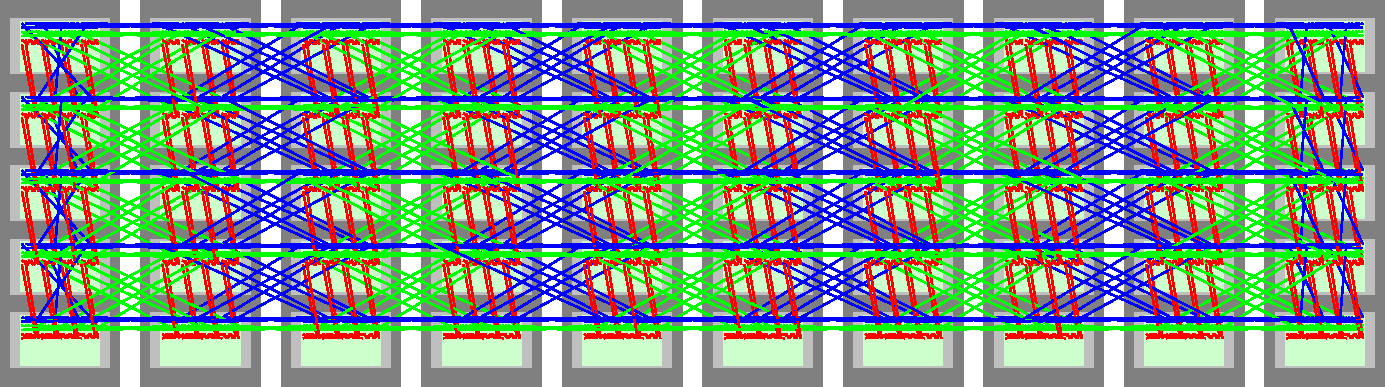
\includegraphics[width=\textwidth]{figures/spinnaker106}
				\caption[SpiNNaker machine mapped into cabinets and racks.]{The largest
				SpiNNaker machine with 1,200 boards ($20\times20$ threeboards) and
				1,036,800 cores mapped into 10 cabinets of 5 racks each.  Coloured lines
				represent wires connecting {\color{red}North/South},
				{\color{green}North-East/South-West} and {\color{blue}East/West} links.}
				\label{fig:spinnaker106}
			\end{figure}
			
			Even though the system is physically several metres long, the longest wire
			will only be around one metre in length which is within the tolerances of
			the high-speed link technology. This placement scheme, therefore, meets
			the wire-length requirement, and due to the use of high-speed serial links
			using commodity cables as described earlier, the wire-cost requirement.
			
		\subsection{Wiring Complexity}
			
			The final concern is that it should not be too complex to
			be installed by hand. The large-scale SpiNNaker machine will contain 3,600
			cables and so it is clearly not practical to have to look up each
			individual connection before wiring it up. Though it is clear that the
			folded arrangement is substantially less regular than the original layout,
			some regularity remains.
			
			By splitting up the wiring tasks by the logical direction (and thus by the
			connector on the board) it is clear that a large amount of regularity
			exists in each group of cables (consider each colour separately in figure
			\ref{fig:spinnaker106}). If the task is further split depending on whether
			the cables stay within a rack or cabinet, batches of identical racks and
			cabinets can be wired up independently before being linked together later.
			For example, the cables connecting North to South (shown in red) remain
			entirely within a cabinet meaning all North/South wiring can be completed
			independently for each cabinet.
			
			Based on the above observations, the connections for all 3,600 cables can
			be described using only 53 instructions rather than 3,200. This satisfies
			the final constraint on wiring complexity.
		
		\subsection{`SpiNNer' Wiring Guide Generator}
			
			As part of this work SpiNNer, a wiring modelling library and wiring guide
			generator, was produced to assist in the construction of SpiNNaker systems
			built from multiple boards. These tools help avoid the error prone process
			of manually visualising the various transformations required during the
			mapping of boards to racks.
			
			The modelling library allows transformations, such as folding, to be
			easily applied to a network of boards. From the transformed network,
			various measurements such as the maximum physical wire length can then be
			directly determined. Using this library the largest SpiNNaker machine can
			be described in 10 lines of code.
			
			The wiring guide generator produces illustrated documents using \LaTeX{}
			which describe the wiring for arbitrarily sized machines\footnote{Many of
			the figures in this section were adapted from wiring guides generated by
			SpiNNer.}. Metrics such as the distribution of wire lengths are included
			along with instructions for wiring the system up. At the time of writing,
			the largest prototype system constructed, a single threeboard, has been
			successfully assembled in a manner consistent with the generated wiring
			guide.
		
		\subsection{Further Work}
			
			% Simplify instructions, alternative wirings.
			
			The wiring guide generator is currently only capable of producing
			exhaustive wiring descriptions with one instruction for each of the 3,600
			cables. The foundations for extracting regularity currently exist in
			experimental form and must eventually be integrated into the wiring guide
			generator.
			
			In addition, further work may be carried out to test alternative wiring
			schemes. In the current scheme, a large proportion of the cables cross
			between different cabinets. As a result a significant amount of the wiring
			cannot be done in isolated batches. An alternative scheme may be able to
			reduce this number and further simplify the task of wiring.
	
	\section{Small-World Super-Computers}
		
		\label{sec:small-world-super-computers}
		
		% In the same way that random search is generic (no free lunch), I tried
		% adding random wires. This is backed up by Watts and Strogatz's small-world
		% network producing algorithm. Built a model. Took into account wiring using
		% techniques in Wiring-Up Super-Computers.
		
		Small-world networks are graphs with a very large number of nodes but,
		within which, the maximum shortest-path length is very small, despite each
		node having a relatively small number of edges. They also contain `clusters'
		of well connected nodes, in contrast with random graphs (which may also
		fulfil the first criterion).
		
		This type of network is often found in nature, perhaps most famously in
		social networks. This property was first observed in 1929 by Hungarian
		author Frigyes Karinthy\cite{karinthy29} and has become popularly known as
		the theory of `six degrees of separation'. This theory states that for any
		two people, chosen at random, there is a chain of at most 6 acquaintances
		which connects them.
		
		This property of maintaining low maximum shortest-path length while still
		remaining locally well connected is desirable for certain computational
		problems. In neural simulations most communication is local but with some
		longer connections existing. The clustering property of small world networks
		means these local connections can be well catered for while the low maximum
		shortest-path length means longer connections are still quick for very large
		models.
		
		\subsection{Network Construction}
		
			Watts and Strogatz have proposed an algorithm for randomly constructing
			networks with small-world properties \cite{watts98}. The algorithm begins
			by creating a ring network with each node connecting to a fixed number of
			its neighbours (figure \ref{fig:ringNetworkB0}). In the next step, with a
			probability of $\beta$, each edge may be replaced by a random connection.
			For $0 < \beta < 1$, the networks produced exhibit varying degrees of the
			small-world properties (figure \ref{fig:ringNetworkB02}).  Finally, in the
			extreme case where $\beta=1$, the network devolves into a random network
			(figure \ref{fig:ringNetworkB1}).
			
			\begin{figure}
				\center
				\begin{subfigure}[t]{0.3\textwidth}
					\center
					\begin{tikzpicture}[thick,inner sep=0.1cm]
	\foreach \t in {30,60,...,360}{
		\node [fill,circle] at (\t:2) {};
		\draw (\t:2) -- (\t+30:2);
		\draw (\t:2) -- (\t+60:2);
	}
\end{tikzpicture}


					\caption{Ring ($\beta = 0.0$)}
					\label{fig:ringNetworkB0}
				\end{subfigure}
				\begin{subfigure}[t]{0.3\textwidth}
					\center
					\newcommand{\mayberandompath}[2]{
	\pgfmathsetmacro{\choice}{random(5)}
	\pgfmathsetmacro{\myrand}{random(12)*30}
	\ifthenelse{\equal{\choice}{1.0}}{
		\draw (#1:2) -- (#2+\myrand:2);
	}{
		\draw (#1:2) -- (#2:2);
	}
}

\begin{tikzpicture}[thick,inner sep=0.1cm]
	\foreach \t in {30,60,...,360}{
		\node [fill,circle] at (\t:2) {};
		\mayberandompath{\t}{\t+30}
		\mayberandompath{\t}{\t+60}
	}
\end{tikzpicture}

					\caption{Watts-Strogatz ($\beta = 0.2$)}
					\label{fig:ringNetworkB02}
				\end{subfigure}
				\begin{subfigure}[t]{0.3\textwidth}
					\center
					\newcommand{\mayberandompath}[2]{
	\pgfmathsetmacro{\myrand}{random(12)*30}
	\draw (#1:2) -- (#2+\myrand:2);
}

\begin{tikzpicture}[thick,inner sep=0.1cm]
	\foreach \t in {30,60,...,360}{
		\node [fill,circle] at (\t:2) {};
		\mayberandompath{\t}{\t+30}
		\mayberandompath{\t}{\t+60}
	}
	
\end{tikzpicture}

					\caption{Random ($\beta = 1.0$)}
					\label{fig:ringNetworkB1}
				\end{subfigure}
				
				\caption{Watts-Strogatz networks with a range of rewiring
				probabilities.}
				\label{fig:ringNetwork}
			\end{figure}
			
			This algorithm is readily extended to torus topologies. In this work, a
			$k$-ary 2-cube (a two dimensional torus $k$ nodes long in each dimension)
			was used as the initial network as in figure \ref{fig:torusNetworkB0}.
			Random permutations are introduced as in the Watts-Strogatz model
			resulting in a network such as figure \ref{fig:torusNetworkB01}.
			
			\begin{figure}
				\center
				\begin{subfigure}[t]{0.45\textwidth}
					\center
					\begin{tikzpicture}[thick,inner sep=0.1cm]
	\clip (-0.5,-0.5) rectangle (5.5,5.5);
	
	\node [fill,circle] (node 146024940) at (0,0) {};
	\node [fill,circle] (node 152407084) at (1,0) {};
	\node [fill,circle] (node 152406988) at (2,0) {};
	\node [fill,circle] (node 152407180) at (3,0) {};
	\node [fill,circle] (node 152407276) at (4,0) {};
	\node [fill,circle] (node 152407404) at (5,0) {};
	\node [fill,circle] (node 152407564) at (0,1) {};
	\node [fill,circle] (node 152407692) at (1,1) {};
	\node [fill,circle] (node 152407724) at (2,1) {};
	\node [fill,circle] (node 152407788) at (3,1) {};
	\node [fill,circle] (node 152407820) at (4,1) {};
	\node [fill,circle] (node 152407948) at (5,1) {};
	\node [fill,circle] (node 152531052) at (0,2) {};
	\node [fill,circle] (node 152531148) at (1,2) {};
	\node [fill,circle] (node 152531180) at (2,2) {};
	\node [fill,circle] (node 152531212) at (3,2) {};
	\node [fill,circle] (node 152531276) at (4,2) {};
	\node [fill,circle] (node 152537548) at (5,2) {};
	\node [fill,circle] (node 152553292) at (0,3) {};
	\node [fill,circle] (node 152553836) at (1,3) {};
	\node [fill,circle] (node 152554092) at (2,3) {};
	\node [fill,circle] (node 152554668) at (3,3) {};
	\node [fill,circle] (node 152554892) at (4,3) {};
	\node [fill,circle] (node 152580172) at (5,3) {};
	\node [fill,circle] (node 152580940) at (0,4) {};
	\node [fill,circle] (node 152581804) at (1,4) {};
	\node [fill,circle] (node 152610924) at (2,4) {};
	\node [fill,circle] (node 152609420) at (3,4) {};
	\node [fill,circle] (node 152656748) at (4,4) {};
	\node [fill,circle] (node 152656844) at (5,4) {};
	\node [fill,circle] (node 152656972) at (0,5) {};
	\node [fill,circle] (node 152657068) at (1,5) {};
	\node [fill,circle] (node 152657100) at (2,5) {};
	\node [fill,circle] (node 152657132) at (3,5) {};
	\node [fill,circle] (node 152657164) at (4,5) {};
	\node [fill,circle] (node 152657260) at (5,5) {};
	
	\draw (node 146024940)
							         .. controls +(0.500000,-1.000000)
							                 and +(0.500000,1.000000)
							         .. (node 152656972);
	\draw (node 146024940)
							         .. controls +(-1.000000,0.500000)
							                 and +(1.000000,0.500000)
							         .. (node 152407404);
	\draw (node 146024940) -- (node 152407084);
	\draw (node 146024940) -- (node 152407564);
	\draw (node 152407084) -- (node 152407692);
	\draw (node 152407084)
							         .. controls +(0.500000,-1.000000)
							                 and +(0.500000,1.000000)
							         .. (node 152657068);
	\draw (node 152406988) -- (node 152407180);
	\draw (node 152406988) -- (node 152407724);
	\draw (node 152406988) -- (node 152407084);
	\draw (node 152406988)
							         .. controls +(0.500000,-1.000000)
							                 and +(0.500000,1.000000)
							         .. (node 152657100);
	\draw (node 152407180)
							         .. controls +(0.500000,-1.000000)
							                 and +(0.500000,1.000000)
							         .. (node 152657132);
	\draw (node 152407180) -- (node 152407276);
	\draw (node 152407180) -- (node 152407788);
	\draw (node 152407276) -- (node 152407404);
	\draw (node 152407276) -- (node 152407820);
	\draw (node 152407276)
							         .. controls +(0.500000,-1.000000)
							                 and +(0.500000,1.000000)
							         .. (node 152657164);
	\draw (node 152407404) -- (node 152407948);
	\draw (node 152407404)
							         .. controls +(0.500000,-1.000000)
							                 and +(0.500000,1.000000)
							         .. (node 152657260);
	\draw (node 152407564)
							         .. controls +(-1.000000,0.500000)
							                 and +(1.000000,0.500000)
							         .. (node 152407948);
	\draw (node 152407564) -- (node 152531052);
	\draw (node 152407564) -- (node 152407692);
	\draw (node 152407692) -- (node 152407724);
	\draw (node 152407692) -- (node 152531148);
	\draw (node 152407724) -- (node 152407788);
	\draw (node 152407724) -- (node 152531180);
	\draw (node 152407788) -- (node 152407820);
	\draw (node 152407788) -- (node 152531212);
	\draw (node 152407820) -- (node 152531276);
	\draw (node 152407820) -- (node 152407948);
	\draw (node 152407948) -- (node 152537548);
	\draw (node 152531052) -- (node 152553292);
	\draw (node 152531052)
							         .. controls +(-1.000000,0.500000)
							                 and +(1.000000,0.500000)
							         .. (node 152537548);
	\draw (node 152531052) -- (node 152531148);
	\draw (node 152531148) -- (node 152553836);
	\draw (node 152531148) -- (node 152531180);
	\draw (node 152531180) -- (node 152554092);
	\draw (node 152531180) -- (node 152531212);
	\draw (node 152531212) -- (node 152531276);
	\draw (node 152531212) -- (node 152554668);
	\draw (node 152531276) -- (node 152537548);
	\draw (node 152531276) -- (node 152554892);
	\draw (node 152537548) -- (node 152580172);
	\draw (node 152553292) -- (node 152580940);
	\draw (node 152553292)
							         .. controls +(-1.000000,0.500000)
							                 and +(1.000000,0.500000)
							         .. (node 152580172);
	\draw (node 152553292) -- (node 152553836);
	\draw (node 152553836) -- (node 152554092);
	\draw (node 152553836) -- (node 152581804);
	\draw (node 152554092) -- (node 152610924);
	\draw (node 152554092) -- (node 152554668);
	\draw (node 152554668) -- (node 152554892);
	\draw (node 152554668) -- (node 152609420);
	\draw (node 152554892) -- (node 152580172);
	\draw (node 152554892) -- (node 152656748);
	\draw (node 152580172) -- (node 152656844);
	\draw (node 152580940)
							         .. controls +(-1.000000,0.500000)
							                 and +(1.000000,0.500000)
							         .. (node 152656844);
	\draw (node 152580940) -- (node 152656972);
	\draw (node 152580940) -- (node 152581804);
	\draw (node 152581804) -- (node 152610924);
	\draw (node 152581804) -- (node 152657068);
	\draw (node 152610924) -- (node 152657100);
	\draw (node 152609420) -- (node 152656748);
	\draw (node 152609420) -- (node 152610924);
	\draw (node 152609420) -- (node 152657132);
	\draw (node 152656748) -- (node 152656844);
	\draw (node 152656748) -- (node 152657164);
	\draw (node 152656844) -- (node 152657260);
	\draw (node 152656972)
							         .. controls +(-1.000000,0.500000)
							                 and +(1.000000,0.500000)
							         .. (node 152657260);
	\draw (node 152656972) -- (node 152657068);
	\draw (node 152657068) -- (node 152657100);
	\draw (node 152657100) -- (node 152657132);
	\draw (node 152657132) -- (node 152657164);
	\draw (node 152657164) -- (node 152657260);
\end{tikzpicture}

					\caption{Unmodified torus ($\beta=0.0$)}
					\label{fig:torusNetworkB0}
				\end{subfigure}
				\begin{subfigure}[t]{0.45\textwidth}
					\center
					\begin{tikzpicture}[thick,inner sep=0.1cm]
	\clip (-0.5,-0.5) rectangle (5.5,5.5);
	
	\node [fill,circle] (node 163015180) at (0,0) {};
	\node [fill,circle] (node 169393228) at (1,0) {};
	\node [fill,circle] (node 169393132) at (2,0) {};
	\node [fill,circle] (node 169393324) at (3,0) {};
	\node [fill,circle] (node 169393420) at (4,0) {};
	\node [fill,circle] (node 169393548) at (5,0) {};
	\node [fill,circle] (node 169393708) at (0,1) {};
	\node [fill,circle] (node 169393836) at (1,1) {};
	\node [fill,circle] (node 169393868) at (2,1) {};
	\node [fill,circle] (node 169393932) at (3,1) {};
	\node [fill,circle] (node 169393964) at (4,1) {};
	\node [fill,circle] (node 169394092) at (5,1) {};
	\node [fill,circle] (node 169521292) at (0,2) {};
	\node [fill,circle] (node 169521388) at (1,2) {};
	\node [fill,circle] (node 169521420) at (2,2) {};
	\node [fill,circle] (node 169521452) at (3,2) {};
	\node [fill,circle] (node 169521516) at (4,2) {};
	\node [fill,circle] (node 169527788) at (5,2) {};
	\node [fill,circle] (node 169543532) at (0,3) {};
	\node [fill,circle] (node 169544076) at (1,3) {};
	\node [fill,circle] (node 169544332) at (2,3) {};
	\node [fill,circle] (node 169544908) at (3,3) {};
	\node [fill,circle] (node 169545132) at (4,3) {};
	\node [fill,circle] (node 169574508) at (5,3) {};
	\node [fill,circle] (node 169575276) at (0,4) {};
	\node [fill,circle] (node 169576140) at (1,4) {};
	\node [fill,circle] (node 169601164) at (2,4) {};
	\node [fill,circle] (node 169599660) at (3,4) {};
	\node [fill,circle] (node 169646988) at (4,4) {};
	\node [fill,circle] (node 169647084) at (5,4) {};
	\node [fill,circle] (node 169647212) at (0,5) {};
	\node [fill,circle] (node 169647308) at (1,5) {};
	\node [fill,circle] (node 169647340) at (2,5) {};
	\node [fill,circle] (node 169647372) at (3,5) {};
	\node [fill,circle] (node 169647404) at (4,5) {};
	\node [fill,circle] (node 169647500) at (5,5) {};
	
	\draw (node 163015180) -- (node 169393228);
	\draw (node 163015180)
							         .. controls +(-1.000000,0.500000)
							                 and +(1.000000,0.500000)
							         .. (node 169393548);
	\draw (node 163015180)
							         .. controls +(0.500000,-1.000000)
							                 and +(0.500000,1.000000)
							         .. (node 169575276);
	\draw (node 163015180)
							         .. controls +(0.500000,-1.000000)
							                 and +(0.500000,1.000000)
							         .. (node 169647212);
	\draw (node 169393228) -- (node 169647500);
	\draw (node 169393228) -- (node 169393836);
	\draw (node 169393228)
							         .. controls +(0.500000,-1.000000)
							                 and +(0.500000,1.000000)
							         .. (node 169647308);
	\draw (node 169393132) -- (node 169393324);
	\draw (node 169393132) -- (node 169393228);
	\draw (node 169393132)
							         .. controls +(0.500000,-1.000000)
							                 and +(0.500000,1.000000)
							         .. (node 169647340);
	\draw (node 169393132) -- (node 169393868);
	\draw (node 169393324)
							         .. controls +(0.500000,-1.000000)
							                 and +(0.500000,1.000000)
							         .. (node 169647372);
	\draw (node 169393324) -- (node 169393420);
	\draw (node 169393324) -- (node 169393932);
	\draw (node 169393420) -- (node 169393548);
	\draw (node 169393420)
							         .. controls +(0.500000,-1.000000)
							                 and +(0.500000,1.000000)
							         .. (node 169521516);
	\draw (node 169393420) -- (node 169393964);
	\draw (node 169393548)
							         .. controls +(0.500000,-1.000000)
							                 and +(0.500000,1.000000)
							         .. (node 169647500);
	\draw (node 169393548) -- (node 169394092);
	\draw (node 169393708)
							         .. controls +(-1.000000,0.500000)
							                 and +(1.000000,0.500000)
							         .. (node 169394092);
	\draw (node 169393708) -- (node 169521292);
	\draw (node 169393708) -- (node 169393836);
	\draw (node 169393836) -- (node 169393868);
	\draw (node 169393836) -- (node 169521388);
	\draw (node 169393836) -- (node 169647340);
	\draw (node 169393868) -- (node 169393932);
	\draw (node 169393932) -- (node 169647212);
	\draw (node 169393932) -- (node 169543532);
	\draw (node 169393932) -- (node 169521452);
	\draw (node 169393932) -- (node 169521516);
	\draw (node 169393964) -- (node 169394092);
	\draw (node 169394092) -- (node 169527788);
	\draw (node 169394092)
							         .. controls +(0.500000,-1.000000)
							                 and +(0.500000,1.000000)
							         .. (node 169647500);
	\draw (node 169521292)
							         .. controls +(-1.000000,0.500000)
							                 and +(1.000000,0.500000)
							         .. (node 169527788);
	\draw (node 169521292) -- (node 169543532);
	\draw (node 169521292) -- (node 169521388);
	\draw (node 169521420) -- (node 169521452);
	\draw (node 169521420) -- (node 169544332);
	\draw (node 169521452) -- (node 169544908);
	\draw (node 169521452) -- (node 169521516);
	\draw (node 169521516) -- (node 169527788);
	\draw (node 169521516) -- (node 169647340);
	\draw (node 169521516) -- (node 169545132);
	\draw (node 169527788) -- (node 169574508);
	\draw (node 169543532) -- (node 169544076);
	\draw (node 169543532) -- (node 169575276);
	\draw (node 169544076) -- (node 169544332);
	\draw (node 169544076) -- (node 169576140);
	\draw (node 169544332) -- (node 169544908);
	\draw (node 169544332) -- (node 169601164);
	\draw (node 169544908) -- (node 169545132);
	\draw (node 169544908) -- (node 169599660);
	\draw (node 169545132) -- (node 169574508);
	\draw (node 169545132) -- (node 169646988);
	\draw (node 169574508) -- (node 169647084);
	\draw (node 169575276)
							         .. controls +(-1.000000,0.500000)
							                 and +(1.000000,0.500000)
							         .. (node 169647084);
	\draw (node 169575276) -- (node 169647212);
	\draw (node 169576140) -- (node 169601164);
	\draw (node 169576140) -- (node 169647308);
	\draw (node 169601164) -- (node 169647340);
	\draw (node 169599660) -- (node 169646988);
	\draw (node 169599660) -- (node 169601164);
	\draw (node 169599660) -- (node 169647372);
	\draw (node 169646988) -- (node 169647084);
	\draw (node 169646988) -- (node 169647404);
	\draw (node 169647212)
							         .. controls +(-1.000000,0.500000)
							                 and +(1.000000,0.500000)
							         .. (node 169647500);
	\draw (node 169647212) -- (node 169647308);
	\draw (node 169647308) -- (node 169647340);
	\draw (node 169647372) -- (node 169647404);
	
\end{tikzpicture}

					\caption{Rewired torus ($\beta=0.1$)}
					\label{fig:torusNetworkB01}
				\end{subfigure}
				
				\caption{Extension of the Watts-Strogatz model to a 6-ary 2-cube.}
				\label{fig:torusNetwork}
			\end{figure}
			
			A $k$-ary $n$-cube has an average shortest path length of $\frac{nk}{4}$.
			This is because a packet travels (on average, under uniform random
			traffic) $\frac{1}{4}$ of the way around each of the $n$, $k$-node-long
			dimensions. In this case, that means the average path length is $\frac{2
			\times 6}{4} = 3$.
			
			By contrast, for the rewired version shown, the average shortest path is
			now reduced to 2.77 hops. As in Watts-Strogatz networks, the average path
			length has been brought down while much of the local connectivity remains.
		
		
		\subsection{Experiments}
			
			Experiments using a simple graph model were carried out to determine the
			effects of rewiring on shortest-path length. Figure
			\ref{fig:smallWorldTorus} shows that the shortest-path length drops
			rapidly but, as more links are rewired, returns quickly diminish. As a
			result, it can be concluded that the amount of rewiring required to
			produce a significant impact on the shortest-path length can be very
			small. These results are similar to the findings of others such as Shin et
			al. who found an increase in bandwidth (but did not test latency) when
			using small-world networks \cite{shin11}.
			
			\begin{figure}
				\center
				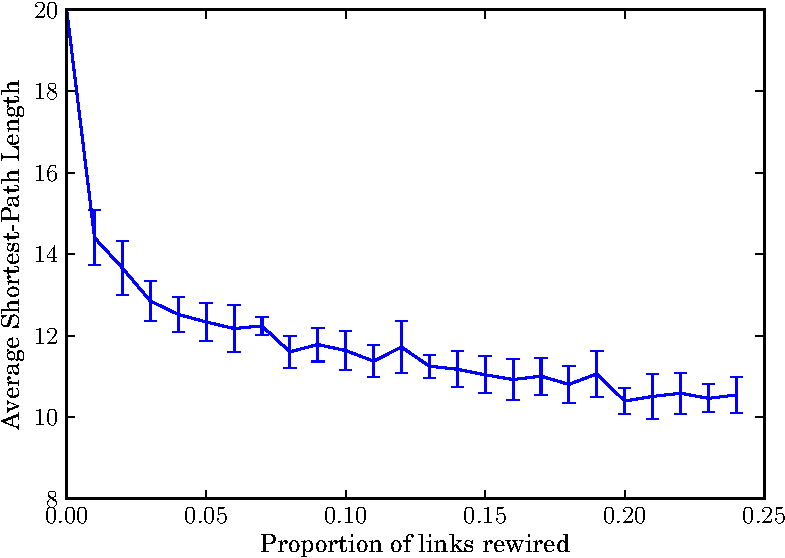
\includegraphics[width=0.7\textwidth]{figures/smallWorldTorus}
				\caption[Average shortest-path length for folded 40-ary 2-cube.]{Average
				shortest-path length for folded 40-ary 2-cube (mean of 10 runs, error
				bars show 1 standard deviation).}
				\label{fig:smallWorldTorus}
			\end{figure}
			
			Unfortunately, random wiring can be problematic for real-world systems.
			As discussed in \S\ref{sec:wiring-up-large-spinnaker-machines}, long wires
			must be avoided for many interconnection technologies and adding random
			wiring can cause many such links to be created. For example, in figure
			\ref{fig:torusNetworkB01} a long wire from the top right node stretches
			almost to the bottom left node.
			
			Work by others such as Koibuchi et al. have attempted to solve this
			problem in completely random topologies \cite{koibuchi13}.  Unfortunately
			their approaches are not applicable to networks which already feature a
			high degree of structure such as the underlying torus network used in
			these experiments. As a result, a new scheme was devised.
			
			To work around this problem, we first fold the network (as discussed
			previously in \S\ref{sec:folding-toroids}) to eliminate the long
			wrap-around wires which connect up the torus (figure
			\ref{fig:torusNetworkFB0}). Next, rewiring is carried out but with a limit
			on the maximum wire length which can be created (figure
			\ref{fig:torusNetworkFB01}).  This rewiring constrains the maximum wire to
			be 3 units long (where a unit is the spacing between each node in a given
			dimension). Even with this limitation on wire length, the maximum path
			length still drops, this time to 2.73 (from 3 in the unwired network), but
			now there are no physically long wires.
			
			\begin{figure}
				\center
				\begin{subfigure}[t]{0.45\textwidth}
					\center
					\begin{tikzpicture}[thick,inner sep=0.1cm]
	\node [fill,circle] (node 172968780) at (0.000000,0.000000) {};
	\node [fill,circle] (node 179346828) at (2.000000,0.000000) {};
	\node [fill,circle] (node 179346732) at (4.000000,0.000000) {};
	\node [fill,circle] (node 179346924) at (5.000000,0.000000) {};
	\node [fill,circle] (node 179347020) at (3.000000,0.000000) {};
	\node [fill,circle] (node 179347148) at (1.000000,0.000000) {};
	\node [fill,circle] (node 179347308) at (0.000000,2.000000) {};
	\node [fill,circle] (node 179347436) at (2.000000,2.000000) {};
	\node [fill,circle] (node 179478572) at (4.000000,2.000000) {};
	\node [fill,circle] (node 179478636) at (5.000000,2.000000) {};
	\node [fill,circle] (node 179478668) at (3.000000,2.000000) {};
	\node [fill,circle] (node 179478796) at (1.000000,2.000000) {};
	\node [fill,circle] (node 179478988) at (0.000000,4.000000) {};
	\node [fill,circle] (node 179479084) at (2.000000,4.000000) {};
	\node [fill,circle] (node 179479116) at (4.000000,4.000000) {};
	\node [fill,circle] (node 179479148) at (5.000000,4.000000) {};
	\node [fill,circle] (node 179479212) at (3.000000,4.000000) {};
	\node [fill,circle] (node 179485484) at (1.000000,4.000000) {};
	\node [fill,circle] (node 179501228) at (0.000000,5.000000) {};
	\node [fill,circle] (node 179501772) at (2.000000,5.000000) {};
	\node [fill,circle] (node 179502028) at (4.000000,5.000000) {};
	\node [fill,circle] (node 179502604) at (5.000000,5.000000) {};
	\node [fill,circle] (node 179502828) at (3.000000,5.000000) {};
	\node [fill,circle] (node 179524012) at (1.000000,5.000000) {};
	\node [fill,circle] (node 179524780) at (0.000000,3.000000) {};
	\node [fill,circle] (node 179525644) at (2.000000,3.000000) {};
	\node [fill,circle] (node 179554764) at (4.000000,3.000000) {};
	\node [fill,circle] (node 179553260) at (5.000000,3.000000) {};
	\node [fill,circle] (node 179604684) at (3.000000,3.000000) {};
	\node [fill,circle] (node 179604780) at (1.000000,3.000000) {};
	\node [fill,circle] (node 179604908) at (0.000000,1.000000) {};
	\node [fill,circle] (node 179605004) at (2.000000,1.000000) {};
	\node [fill,circle] (node 179605036) at (4.000000,1.000000) {};
	\node [fill,circle] (node 179605068) at (5.000000,1.000000) {};
	\node [fill,circle] (node 179605100) at (3.000000,1.000000) {};
	\node [fill,circle] (node 179605196) at (1.000000,1.000000) {};
	
	\draw (node 172968780) -- (node 179347148);
	\draw (node 172968780) -- (node 179604908);
	\draw (node 172968780)
							         .. controls +(1.000000,0.500000)
							                 and +(-1.000000,0.500000)
							         .. (node 179346828);
	\draw (node 172968780)
							         .. controls +(0.500000,1.000000)
							                 and +(0.500000,-1.000000)
							         .. (node 179347308);
	\draw (node 179346828)
							         .. controls +(0.500000,1.000000)
							                 and +(0.500000,-1.000000)
							         .. (node 179347436);
	\draw (node 179346828) -- (node 179605004);
	\draw (node 179346732) -- (node 179346924);
	\draw (node 179346732)
							         .. controls +(-1.000000,0.500000)
							                 and +(1.000000,0.500000)
							         .. (node 179346828);
	\draw (node 179346732) -- (node 179605036);
	\draw (node 179346732)
							         .. controls +(0.500000,1.000000)
							                 and +(0.500000,-1.000000)
							         .. (node 179478572);
	\draw (node 179346924) -- (node 179605068);
	\draw (node 179346924)
							         .. controls +(-1.000000,0.500000)
							                 and +(1.000000,0.500000)
							         .. (node 179347020);
	\draw (node 179346924)
							         .. controls +(0.500000,1.000000)
							                 and +(0.500000,-1.000000)
							         .. (node 179478636);
	\draw (node 179347020)
							         .. controls +(-1.000000,0.500000)
							                 and +(1.000000,0.500000)
							         .. (node 179347148);
	\draw (node 179347020)
							         .. controls +(0.500000,1.000000)
							                 and +(0.500000,-1.000000)
							         .. (node 179478668);
	\draw (node 179347020) -- (node 179605100);
	\draw (node 179347148) -- (node 179605196);
	\draw (node 179347148)
							         .. controls +(0.500000,1.000000)
							                 and +(0.500000,-1.000000)
							         .. (node 179478796);
	\draw (node 179347308) -- (node 179478796);
	\draw (node 179347308)
							         .. controls +(1.000000,0.500000)
							                 and +(-1.000000,0.500000)
							         .. (node 179347436);
	\draw (node 179347308)
							         .. controls +(0.500000,1.000000)
							                 and +(0.500000,-1.000000)
							         .. (node 179478988);
	\draw (node 179347436)
							         .. controls +(1.000000,0.500000)
							                 and +(-1.000000,0.500000)
							         .. (node 179478572);
	\draw (node 179347436)
							         .. controls +(0.500000,1.000000)
							                 and +(0.500000,-1.000000)
							         .. (node 179479084);
	\draw (node 179478572)
							         .. controls +(0.500000,1.000000)
							                 and +(0.500000,-1.000000)
							         .. (node 179479116);
	\draw (node 179478572) -- (node 179478636);
	\draw (node 179478636)
							         .. controls +(-1.000000,0.500000)
							                 and +(1.000000,0.500000)
							         .. (node 179478668);
	\draw (node 179478636)
							         .. controls +(0.500000,1.000000)
							                 and +(0.500000,-1.000000)
							         .. (node 179479148);
	\draw (node 179478668)
							         .. controls +(-1.000000,0.500000)
							                 and +(1.000000,0.500000)
							         .. (node 179478796);
	\draw (node 179478668)
							         .. controls +(0.500000,1.000000)
							                 and +(0.500000,-1.000000)
							         .. (node 179479212);
	\draw (node 179478796)
							         .. controls +(0.500000,1.000000)
							                 and +(0.500000,-1.000000)
							         .. (node 179485484);
	\draw (node 179478988) -- (node 179485484);
	\draw (node 179478988) -- (node 179501228);
	\draw (node 179478988)
							         .. controls +(1.000000,0.500000)
							                 and +(-1.000000,0.500000)
							         .. (node 179479084);
	\draw (node 179479084)
							         .. controls +(1.000000,0.500000)
							                 and +(-1.000000,0.500000)
							         .. (node 179479116);
	\draw (node 179479084) -- (node 179501772);
	\draw (node 179479116) -- (node 179479148);
	\draw (node 179479116) -- (node 179502028);
	\draw (node 179479148) -- (node 179502604);
	\draw (node 179479148)
							         .. controls +(-1.000000,0.500000)
							                 and +(1.000000,0.500000)
							         .. (node 179479212);
	\draw (node 179479212)
							         .. controls +(-1.000000,0.500000)
							                 and +(1.000000,0.500000)
							         .. (node 179485484);
	\draw (node 179479212) -- (node 179502828);
	\draw (node 179485484) -- (node 179524012);
	\draw (node 179501228) -- (node 179524012);
	\draw (node 179501228)
							         .. controls +(0.500000,-1.000000)
							                 and +(0.500000,1.000000)
							         .. (node 179524780);
	\draw (node 179501228)
							         .. controls +(1.000000,0.500000)
							                 and +(-1.000000,0.500000)
							         .. (node 179501772);
	\draw (node 179501772)
							         .. controls +(1.000000,0.500000)
							                 and +(-1.000000,0.500000)
							         .. (node 179502028);
	\draw (node 179501772)
							         .. controls +(0.500000,-1.000000)
							                 and +(0.500000,1.000000)
							         .. (node 179525644);
	\draw (node 179502028) -- (node 179502604);
	\draw (node 179502028)
							         .. controls +(0.500000,-1.000000)
							                 and +(0.500000,1.000000)
							         .. (node 179554764);
	\draw (node 179502604)
							         .. controls +(-1.000000,0.500000)
							                 and +(1.000000,0.500000)
							         .. (node 179502828);
	\draw (node 179502604)
							         .. controls +(0.500000,-1.000000)
							                 and +(0.500000,1.000000)
							         .. (node 179553260);
	\draw (node 179502828)
							         .. controls +(0.500000,-1.000000)
							                 and +(0.500000,1.000000)
							         .. (node 179604684);
	\draw (node 179502828)
							         .. controls +(-1.000000,0.500000)
							                 and +(1.000000,0.500000)
							         .. (node 179524012);
	\draw (node 179524012)
							         .. controls +(0.500000,-1.000000)
							                 and +(0.500000,1.000000)
							         .. (node 179604780);
	\draw (node 179524780)
							         .. controls +(0.500000,-1.000000)
							                 and +(0.500000,1.000000)
							         .. (node 179604908);
	\draw (node 179524780) -- (node 179604780);
	\draw (node 179524780)
							         .. controls +(1.000000,0.500000)
							                 and +(-1.000000,0.500000)
							         .. (node 179525644);
	\draw (node 179525644)
							         .. controls +(1.000000,0.500000)
							                 and +(-1.000000,0.500000)
							         .. (node 179554764);
	\draw (node 179525644)
							         .. controls +(0.500000,-1.000000)
							                 and +(0.500000,1.000000)
							         .. (node 179605004);
	\draw (node 179554764)
							         .. controls +(0.500000,-1.000000)
							                 and +(0.500000,1.000000)
							         .. (node 179605036);
	\draw (node 179553260)
							         .. controls +(0.500000,-1.000000)
							                 and +(0.500000,1.000000)
							         .. (node 179605068);
	\draw (node 179553260)
							         .. controls +(-1.000000,0.500000)
							                 and +(1.000000,0.500000)
							         .. (node 179604684);
	\draw (node 179553260) -- (node 179554764);
	\draw (node 179604684)
							         .. controls +(-1.000000,0.500000)
							                 and +(1.000000,0.500000)
							         .. (node 179604780);
	\draw (node 179604684)
							         .. controls +(0.500000,-1.000000)
							                 and +(0.500000,1.000000)
							         .. (node 179605100);
	\draw (node 179604780)
							         .. controls +(0.500000,-1.000000)
							                 and +(0.500000,1.000000)
							         .. (node 179605196);
	\draw (node 179604908) -- (node 179605196);
	\draw (node 179604908)
							         .. controls +(1.000000,0.500000)
							                 and +(-1.000000,0.500000)
							         .. (node 179605004);
	\draw (node 179605004)
							         .. controls +(1.000000,0.500000)
							                 and +(-1.000000,0.500000)
							         .. (node 179605036);
	\draw (node 179605036) -- (node 179605068);
	\draw (node 179605068)
							         .. controls +(-1.000000,0.500000)
							                 and +(1.000000,0.500000)
							         .. (node 179605100);
	\draw (node 179605100)
							         .. controls +(-1.000000,0.500000)
							                 and +(1.000000,0.500000)
							         .. (node 179605196);
	
\end{tikzpicture}

					\caption{Folded torus ($\beta=0.0$)}
					\label{fig:torusNetworkFB0}
				\end{subfigure}
				\begin{subfigure}[t]{0.45\textwidth}
					\center
					\begin{tikzpicture}[thick,inner sep=0.1cm]
	\node [fill,circle] (node 149404876) at (0.000000,0.000000) {};
	\node [fill,circle] (node 155782924) at (2.000000,0.000000) {};
	\node [fill,circle] (node 155782828) at (4.000000,0.000000) {};
	\node [fill,circle] (node 155783020) at (5.000000,0.000000) {};
	\node [fill,circle] (node 155783116) at (3.000000,0.000000) {};
	\node [fill,circle] (node 155910252) at (1.000000,0.000000) {};
	\node [fill,circle] (node 155910412) at (0.000000,2.000000) {};
	\node [fill,circle] (node 155910540) at (2.000000,2.000000) {};
	\node [fill,circle] (node 155910572) at (4.000000,2.000000) {};
	\node [fill,circle] (node 155910636) at (5.000000,2.000000) {};
	\node [fill,circle] (node 155910668) at (3.000000,2.000000) {};
	\node [fill,circle] (node 155910796) at (1.000000,2.000000) {};
	\node [fill,circle] (node 155910988) at (0.000000,4.000000) {};
	\node [fill,circle] (node 155911084) at (2.000000,4.000000) {};
	\node [fill,circle] (node 155911116) at (4.000000,4.000000) {};
	\node [fill,circle] (node 155911148) at (5.000000,4.000000) {};
	\node [fill,circle] (node 155911212) at (3.000000,4.000000) {};
	\node [fill,circle] (node 155921580) at (1.000000,4.000000) {};
	\node [fill,circle] (node 155937324) at (0.000000,5.000000) {};
	\node [fill,circle] (node 155937868) at (2.000000,5.000000) {};
	\node [fill,circle] (node 155938124) at (4.000000,5.000000) {};
	\node [fill,circle] (node 155938700) at (5.000000,5.000000) {};
	\node [fill,circle] (node 155959436) at (3.000000,5.000000) {};
	\node [fill,circle] (node 155960108) at (1.000000,5.000000) {};
	\node [fill,circle] (node 155960876) at (0.000000,3.000000) {};
	\node [fill,circle] (node 155961740) at (2.000000,3.000000) {};
	\node [fill,circle] (node 155990860) at (4.000000,3.000000) {};
	\node [fill,circle] (node 155989356) at (5.000000,3.000000) {};
	\node [fill,circle] (node 156040780) at (3.000000,3.000000) {};
	\node [fill,circle] (node 156040876) at (1.000000,3.000000) {};
	\node [fill,circle] (node 156041004) at (0.000000,1.000000) {};
	\node [fill,circle] (node 156041100) at (2.000000,1.000000) {};
	\node [fill,circle] (node 156041132) at (4.000000,1.000000) {};
	\node [fill,circle] (node 156041164) at (5.000000,1.000000) {};
	\node [fill,circle] (node 156041196) at (3.000000,1.000000) {};
	\node [fill,circle] (node 156074092) at (1.000000,1.000000) {};
	
	\draw (node 149404876) -- (node 155910252);
	\draw (node 149404876)
							         .. controls +(1.000000,0.500000)
							                 and +(-1.000000,0.500000)
							         .. (node 155783116);
	\draw (node 149404876)
							         .. controls +(0.500000,1.000000)
							                 and +(0.500000,-1.000000)
							         .. (node 155910412);
	\draw (node 149404876) -- (node 156041004);
	\draw (node 155782924)
							         .. controls +(0.500000,1.000000)
							                 and +(0.500000,-1.000000)
							         .. (node 155910540);
	\draw (node 155782828) -- (node 155783020);
	\draw (node 155782828)
							         .. controls +(0.500000,1.000000)
							                 and +(0.500000,-1.000000)
							         .. (node 155910572);
	\draw (node 155782828)
							         .. controls +(-1.000000,0.500000)
							                 and +(1.000000,0.500000)
							         .. (node 155782924);
	\draw (node 155782828) -- (node 156041132);
	\draw (node 155783020)
							         .. controls +(-1.000000,0.500000)
							                 and +(1.000000,0.500000)
							         .. (node 155783116);
	\draw (node 155783020)
							         .. controls +(0.500000,1.000000)
							                 and +(0.500000,-1.000000)
							         .. (node 155910636);
	\draw (node 155783020) -- (node 156041164);
	\draw (node 155783116)
							         .. controls +(-1.000000,0.500000)
							                 and +(1.000000,0.500000)
							         .. (node 155910252);
	\draw (node 155783116) -- (node 156041196);
	\draw (node 155783116)
							         .. controls +(0.500000,1.000000)
							                 and +(0.500000,-1.000000)
							         .. (node 155910668);
	\draw (node 155910252)
							         .. controls +(0.500000,1.000000)
							                 and +(0.500000,-1.000000)
							         .. (node 155910796);
	\draw (node 155910252) -- (node 156074092);
	\draw (node 155910412)
							         .. controls +(0.500000,1.000000)
							                 and +(0.500000,-1.000000)
							         .. (node 155910988);
	\draw (node 155910412)
							         .. controls +(1.000000,0.500000)
							                 and +(-1.000000,0.500000)
							         .. (node 155910540);
	\draw (node 155910540)
							         .. controls +(1.000000,0.500000)
							                 and +(-1.000000,0.500000)
							         .. (node 155910572);
	\draw (node 155910540)
							         .. controls +(0.500000,1.000000)
							                 and +(0.500000,-1.000000)
							         .. (node 155911084);
	\draw (node 155910572)
							         .. controls +(0.500000,1.000000)
							                 and +(0.500000,-1.000000)
							         .. (node 155911116);
	\draw (node 155910636) -- (node 156041132);
	\draw (node 155910636)
							         .. controls +(0.500000,1.000000)
							                 and +(0.500000,-1.000000)
							         .. (node 155938700);
	\draw (node 155910636)
							         .. controls +(0.500000,1.000000)
							                 and +(0.500000,-1.000000)
							         .. (node 155911148);
	\draw (node 155910668)
							         .. controls +(-1.000000,0.500000)
							                 and +(1.000000,0.500000)
							         .. (node 155910796);
	\draw (node 155910668)
							         .. controls +(0.500000,1.000000)
							                 and +(0.500000,-1.000000)
							         .. (node 155911212);
	\draw (node 155910796) -- (node 156040780);
	\draw (node 155910796)
							         .. controls +(0.500000,1.000000)
							                 and +(0.500000,-1.000000)
							         .. (node 155921580);
	\draw (node 155910988) -- (node 155921580);
	\draw (node 155910988)
							         .. controls +(1.000000,0.500000)
							                 and +(-1.000000,0.500000)
							         .. (node 155911084);
	\draw (node 155911084) -- (node 155990860);
	\draw (node 155911084)
							         .. controls +(1.000000,0.500000)
							                 and +(-1.000000,0.500000)
							         .. (node 155911116);
	\draw (node 155911084) -- (node 155937324);
	\draw (node 155911116) -- (node 155938124);
	\draw (node 155911116) -- (node 155911148);
	\draw (node 155911148)
							         .. controls +(-1.000000,0.500000)
							                 and +(1.000000,0.500000)
							         .. (node 155911212);
	\draw (node 155911212) -- (node 155990860);
	\draw (node 155911212) -- (node 155959436);
	\draw (node 155921580) -- (node 155960108);
	\draw (node 155937324) -- (node 155960108);
	\draw (node 155937324)
							         .. controls +(0.500000,-1.000000)
							                 and +(0.500000,1.000000)
							         .. (node 155960876);
	\draw (node 155937868)
							         .. controls +(1.000000,0.500000)
							                 and +(-1.000000,0.500000)
							         .. (node 155938124);
	\draw (node 155937868)
							         .. controls +(0.500000,-1.000000)
							                 and +(0.500000,1.000000)
							         .. (node 155961740);
	\draw (node 155937868) -- (node 156040876);
	\draw (node 155937868) -- (node 155960108);
	\draw (node 155938124)
							         .. controls +(0.500000,-1.000000)
							                 and +(0.500000,1.000000)
							         .. (node 155990860);
	\draw (node 155938124) -- (node 155938700);
	\draw (node 155938700) -- (node 155938700);
	\draw (node 155938700)
							         .. controls +(-1.000000,0.500000)
							                 and +(1.000000,0.500000)
							         .. (node 155959436);
	\draw (node 155938700)
							         .. controls +(0.500000,-1.000000)
							                 and +(0.500000,1.000000)
							         .. (node 155989356);
	\draw (node 155959436)
							         .. controls +(0.500000,-1.000000)
							                 and +(0.500000,1.000000)
							         .. (node 156040780);
	\draw (node 155959436)
							         .. controls +(-1.000000,0.500000)
							                 and +(1.000000,0.500000)
							         .. (node 155960108);
	\draw (node 155960108)
							         .. controls +(0.500000,-1.000000)
							                 and +(0.500000,1.000000)
							         .. (node 156040876);
	\draw (node 155960876) -- (node 156040876);
	\draw (node 155960876)
							         .. controls +(0.500000,-1.000000)
							                 and +(0.500000,1.000000)
							         .. (node 156041004);
	\draw (node 155960876)
							         .. controls +(1.000000,0.500000)
							                 and +(-1.000000,0.500000)
							         .. (node 155961740);
	\draw (node 155961740)
							         .. controls +(1.000000,0.500000)
							                 and +(-1.000000,0.500000)
							         .. (node 155990860);
	\draw (node 155961740)
							         .. controls +(0.500000,-1.000000)
							                 and +(0.500000,1.000000)
							         .. (node 156041100);
	\draw (node 155989356)
							         .. controls +(-1.000000,0.500000)
							                 and +(1.000000,0.500000)
							         .. (node 156040780);
	\draw (node 155989356) -- (node 155990860);
	\draw (node 155989356)
							         .. controls +(0.500000,-1.000000)
							                 and +(0.500000,1.000000)
							         .. (node 156041164);
	\draw (node 156040780)
							         .. controls +(-1.000000,0.500000)
							                 and +(1.000000,0.500000)
							         .. (node 156040876);
	\draw (node 156040780)
							         .. controls +(0.500000,-1.000000)
							                 and +(0.500000,1.000000)
							         .. (node 156041196);
	\draw (node 156040876)
							         .. controls +(0.500000,-1.000000)
							                 and +(0.500000,1.000000)
							         .. (node 156074092);
	\draw (node 156041004) -- (node 156074092);
	\draw (node 156041004)
							         .. controls +(1.000000,0.500000)
							                 and +(-1.000000,0.500000)
							         .. (node 156041100);
	\draw (node 156041100)
							         .. controls +(1.000000,0.500000)
							                 and +(-1.000000,0.500000)
							         .. (node 156041132);
	\draw (node 156041132) -- (node 156041164);
	\draw (node 156041164)
							         .. controls +(-1.000000,0.500000)
							                 and +(1.000000,0.500000)
							         .. (node 156041196);
	\draw (node 156041196)
							         .. controls +(-1.000000,0.500000)
							                 and +(1.000000,0.500000)
							         .. (node 156074092);
	
\end{tikzpicture}


					\caption{Rewired torus ($\beta=0.1$)}
					\label{fig:torusNetworkFB01}
				\end{subfigure}
				
				\caption{Rewiring a folded torus with constrained maximum wire-length.}
				\label{fig:torusNetworkF}
			\end{figure}
			
			To test the effects of limiting wire lengths when re-wiring, a parameter
			sweep was carried out for a 40-ary 2-cube. The test was carried out after
			folding once and twice in each dimension and finally when the
			network was not folded. The results are given in figure
			\ref{fig:smallWorldLimitedWiring}.
			
			\begin{figure}
				\center
				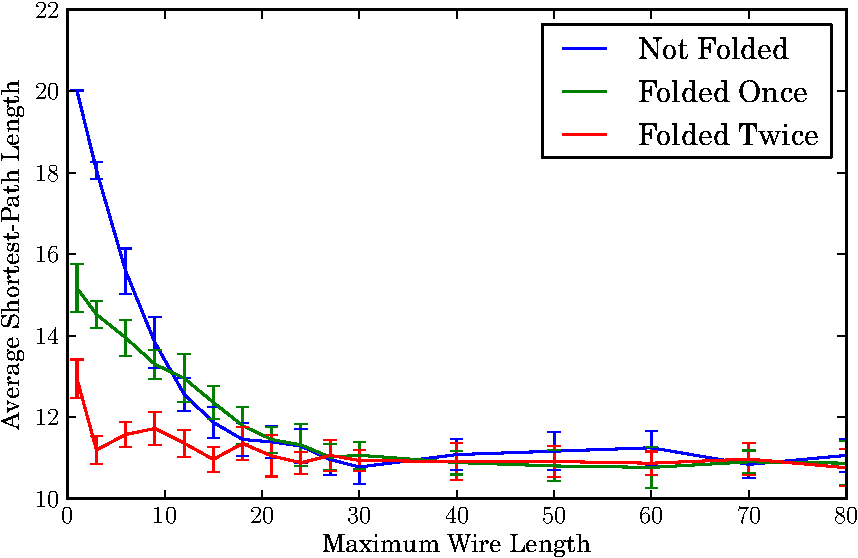
\includegraphics[width=0.7\textwidth]{figures/smallWorldLimitedWiring}
				\caption{Average shortest-path length for folded 40-ary 2-cube with 1\% rewiring}
				\label{fig:smallWorldLimitedWiring}
			\end{figure}
			
			It is clear that when wire lengths are most limited, the average
			shortest-path length improves when the network has been folded. This
			result is intuitive because after folding, physically neighbouring boards
			are no-longer logically adjacent but instead are at opposite ends of the
			system. As a result, limiting wire lengths essentially `prefers' the
			creation of logically longer links which are most likely to pull the
			average path length down.
			
			The other interesting effect is that, above a certain threshold, allowing
			longer wires has no significant effect on the average shortest-path
			length. This may be because wires which stretch further than half-way
			($\frac{k}{2}$ hops) along a given axis could be just as easily reached by
			travelling the shorter distance the other way around the axis. This
			longest useful wire length can be calculated as follows:
			\[
				\textrm{Maximum Useful Wire Length}
					= \sqrt{n \left({\frac{k}{2}}\right)^2}
					= \frac{k\sqrt{n}}{2}
			\]
			For a 40-ary 2-cube the maximum useful wire length is $20\sqrt{2} \approx
			28.3$ which can be visually confirmed in the figure.
		
		\subsection{Further Work}
			
			% Must try this with SpiNNaker topology and racks (maybe even better). Would
			% like to formalise the result into a formula.
			
			% When wire lengths are constrained, the uniformity of the connectivity in
			% the system is reduced.
			
			Figure \ref{fig:ringNetworkLimitedWires} shows valid random links in a
			small ring network with limited wire lengths. Nodes near the top and
			bottom of the ring potentially have shorter average path lengths to all
			other nodes than nodes near the left and right of the ring. This is
			because the allowed random links for top and bottom nodes connect nodes at
			greater logical distances in the ring than those allowed on the left and
			right. The result is that the average path length from two different nodes
			becomes non-uniform across nodes in different parts of the system.
			
			\begin{figure}
				\center
				\begin{tikzpicture}[thick,inner sep=0.1cm]
	\foreach [count=\n] \t in {30,60,...,360}{
		\node [fill,circle] at (90-\t:2) (node \n) {};
		\draw [help lines] (\t:2) -- (\t+30:2);
	}
	
	\draw (node 8) to (node 10);
	\draw (node 8) to (node 11);
	
	\draw (node 7) to (node 11);
	\draw (node 7) to (node 12);
	
	\draw (node 6) to (node 12);
	\draw (node 6) to (node 1);
	
	\draw (node 5) to (node 1);
	\draw (node 5) to (node 2);
	
	\draw (node 4) to (node 2);
	
\end{tikzpicture}


				\caption[Valid random links in a folded ring network with short
				wires.]{Valid random links in ring network when wires limited to a
				length of 1 unit and the network is folded as in figure
				\ref{fig:folding}.}
				\label{fig:ringNetworkLimitedWires}
			\end{figure}
			
			Further work may study the effects of this non-uniformity of average path
			length. The effects of the non-uniformity may be reduced by using greater
			degrees of folding or higher dimensional topologies. In addition, real
			systems are constrained to standard cabinets and racks, as in
			\S\ref{sec:mapping-spinnaker-to-cabinets}, which may change distribution
			of average path lengths in the system.
			
			This work could be extended to include this final mapping into more
			realistic physical placements, for example by building on the SpiNNer
			wiring modelling library. It is anticipated that the more complex
			placements resulting from higher-dimensions and realistic placement will
			result in a more uniform distribution of average path lengths.
	
	%\section{Place and Route}
	%	
	%	Tests written for the Place and Route system for SpiNNaker-103. Gained some
	%	experience with the task. 
	%	
	%	\subsection{Potential Improvements}
	%		
	%		The algorithms used for placement and routing are naive: generally greedy
	%		algorithms.



